\documentclass{article}

\usepackage[margin = 2.5 cm]{geometry}
\usepackage[utf8x]{inputenc}
\usepackage{graphicx}
\usepackage[magyar]{babel}
\usepackage{amsmath}
\usepackage{amsfonts}
\usepackage{booktabs}
\usepackage{mathrsfs}
\usepackage{float}
\usepackage{multirow}
\usepackage{mathtools} 



\begin{document}
	\begin{titlepage}	
		%címlap
		\vspace*{5 cm}
		\begin{center}
			\Huge \textbf{Tárgymanipuláció kulcspontok detektálásán alapuló képfeldolgozással}
			\LARGE
			
			Diplomaterv I. beszámoló\\
			\vspace{12pt} \normalsize
			Ayhan Dániel\\
			LIIAE1
		\end{center}
		\vspace{6 cm}
		Témavezető:\\
		\\		
		Dr. Kiss Bálint
		\begin{center}		
			\vfill
			Budapest, \today	
		\end{center}
	\end{titlepage}
	\newpage
	
	\thispagestyle{empty}
	\tableofcontents
	
	\setlength{\parindent}{0 em}	
	\setlength{\parskip}{1em}
	
	\newpage
	\setcounter{page}{1}
	\section{Bevezetés, feladatkitűzés}
	Az automatizált/robotizált megoldások egyre inkább elterjednek a mindennapi életünkben. Ennek egyik részterülete az olyan robotok kutatása, amelyek az ember otthonában képesek különböző feladatokat végrehajtani, például tárgyakat lokalizálni, megfogni, és áthelyezni. Egy alkalmazása lehet ennek, amikor a robot mozgáskorlátozott, vagy idős embereknek tárgyakat visz oda.
	
	Tetszőleges tárgyak megtalálásához az egyik elterjedt módszer a vizuális információ felhasználása, képfeldolgozás használata.
	
	A feladatom egy tetszőleges tárgy lokalizálására alkalmas algoritmus fejlesztése volt képfeldolgozás segítségével. Lokalizálás alatt a tárgy pontos pozícióját és orientációját, azaz \textit{helyzetét} értem. A tárgyról előzetesen bármilyen információnk lehet, célszerű erre az adathalmazra is képfeldolgozással szert tenni. Feladat volt továbbá, hogy a tanszéki robotlaborban található robotkarral az adott tárgyat meg is fogjam, vagyis a képfeldolgozás információit felhasználó tárgymanipuláló algoritmust fejlesszek.
	
	A tárgymanipulációhoz a robot és a kamera közötti transzformáció meghatározására, vagyis a kéz-szem kalibráció elvégzésére volt szükség.
	
	A 3D pozíció meghatározására szolgáló algoritmussal már korábban foglalkoztam, ebben a beszámolóban a robot-PC interfész megvalósításáról, és a kéz-szem kalibrációról van szó.
	
	\section{A robotirányító rendszer felépítése}
	A robotlaborban a kommunikációs lánc a következő elemekből épül fel:
	
\begin{enumerate}
\item PC
\item PLC (Q03UDVCPU)
\item Robotvezérlő modul (Q172DRCPU)
\item Robotkar (Melfa RV-2F-Q)
\end{enumerate}	

	A kommunikáció a következő módon valósul meg. A PC és PLC között a kommunikáció Modbus/TCP kapcsolaton keresztül történik, a PLC a belső hálózaton DHCP-vel kiosztott statikus IP-n elérhető. A Modbus/TCP egy Ethernet-alapú kommunikációs protokoll, amelyben a szerver elérhetővé teszi a hozzá csatlakozott kliensek számára a regisztereit, azok szabadon írhatók. A PLC és a robotvezérlő modul megosztott memórián keresztül kommunikálnak. A robotvezérlő közvetlenül irányítja a robotkart, azzal egy komplett berendezést alkot, a köztük lévő kommunikáció megoldása nem a felhasználó feladata.
	
%\begin{figure}[H]
%\centering
%\includegraphics[width=\linewidth]{system.png}
%\caption{A robotirányító rendszer felépítése}
%\label{img-gui}
%\end{figure}
	
	\newpage
	A robot megfogójára egy Logitech c525 típusú webkamera van szerelve, ez szolgáltatja a képfeldolgozás számára a vizuális információt.
	
	
%\begin{figure}[H]
%\centering
%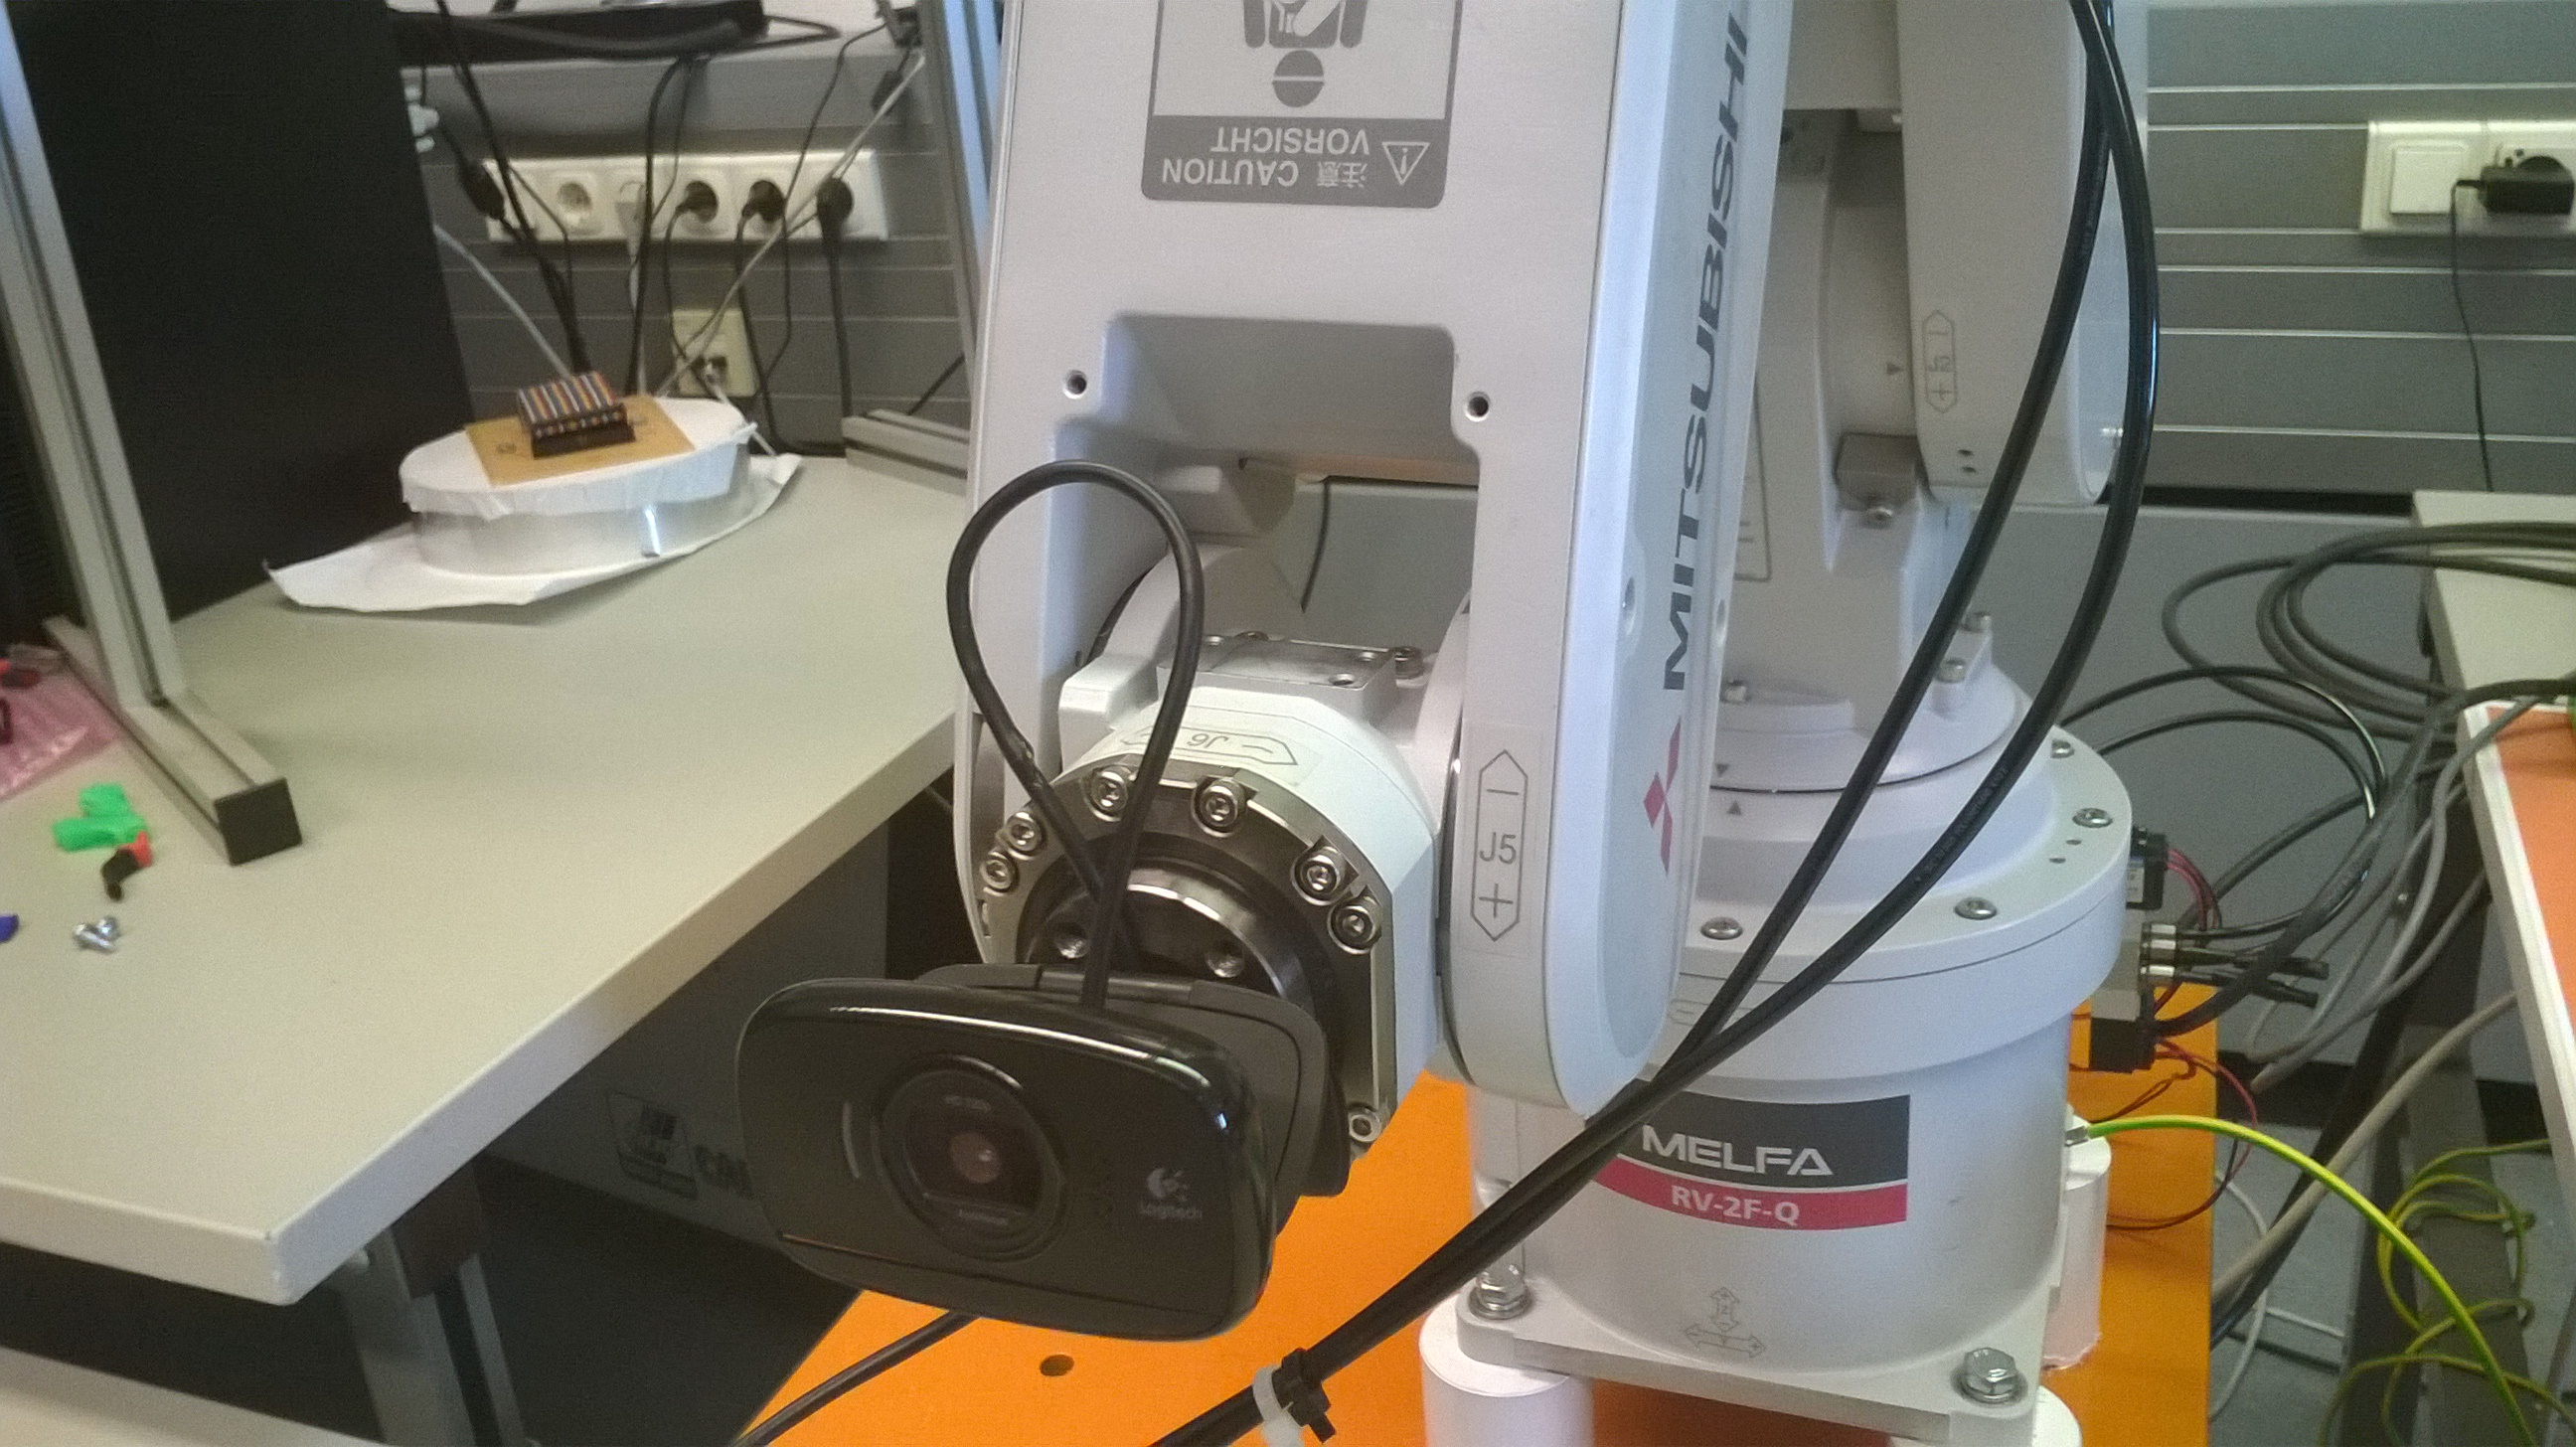
\includegraphics[width=\linewidth]{robocam.jpg}
%\caption{A robotra szerelt kamera}
%\end{figure}
	
	\section{A PLC és robotprogram}
	
	A PLC-n két, a működéshez szükséges program fut. Az egyik egy Modbus szerver, ami a PC-vel való kommunikációt kezeli. Ez a Mitsubishi cég (és a programot korábban felfedező és használó hallgatók) jóvoltából már rendelkezésre állt számomra. 
	
	A másik program a robot felé történő kommunikációért felelős. Minthogy a PLC csak összekötő szerepet játszik a robot és a PC között, ezért ennek a programnak a feladatköre arra korlátozódik, hogy a Modbus-on keresztül kapott értékeket továbbítsa a megosztott memóriába. Ezt a programot Menyhárt Balázs MSc hallgató készítette, én minimális módosításokkal az ő programját használom.
	
	A roboton futó program kiolvassa a megosztott memóriából a megfelelő értékeket, és ennek megfelelően mozgatja a robotkart. Ennek a megvalósítása úgy történik, hogy egy-egy regiszterben kerül átadásra a pozíció-orientáció 6 paramétere. A robotprogram elvégzi a megfelelő korrekciókat (szög-radián átváltás), majd a megadott helyzetbe irányítja a megfogót. Ez ki van még egészítve egy utasításszámlálóval, amelynek értékét a PC-n futó programban vizsgálva megtudhatjuk, hogy az adott utasítást a robot elvégezte-e már.
	\newpage
	\section{A PC program}
	
	A PC program Python nyelven íródott. Képfeldolgozásra az OpenCV függvénykönyvtárat, a Modbus kommunikáció megvalósításához a PyModbusTCP könyvtárat használtam. A program feladata a robot felső szintű vezérlése, azaz célpozíciójának megadása, illetve a kamera kezelése. A legmagasabb szintű funkciója a kéz-szem kalibráció automatikus elvégzése. Az automatikus működésen túl meg lehet adni manuálisan is pozíciót, ahova a robotot mozgatni szeretnénk, valamint manuálisan is lehet képet készíteni a kamerával.
	
	
%\begin{figure}[H]
%\centering
%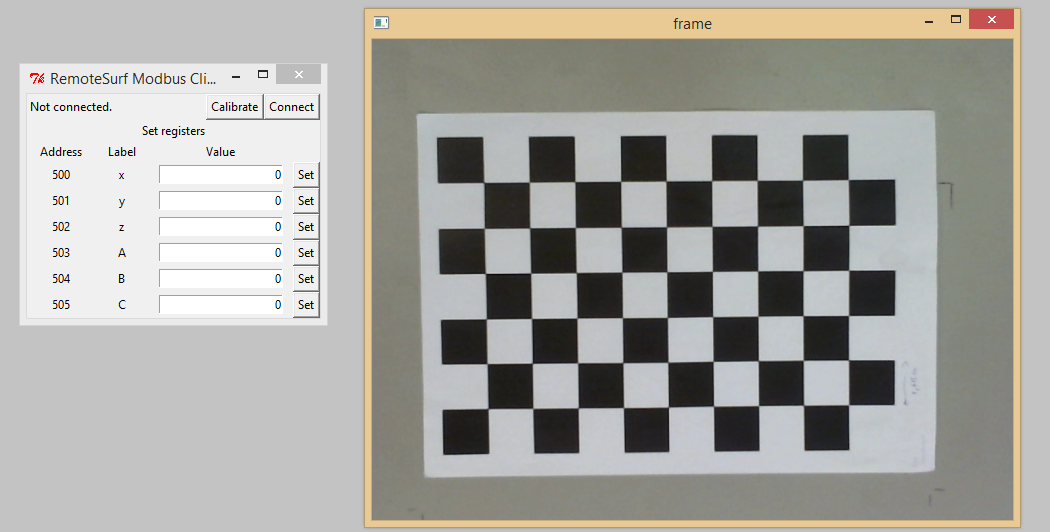
\includegraphics[width=\linewidth]{gui.png}
%\caption{A program felhasználói felülete}
%\label{img-gui}
%\end{figure}

\newpage
	\section{A gépi látás alapfogalmai}
	A kalibrációs algoritmus áttekintése előtt ismerkedjünk meg a gépi látásban, képfeldolgozásban használatos fogalmakkal. A kamerát úgynevezett pinhole-kameramodellel írjuk le. Ez a modell azt feltételezi, hogy a kép keletkezése olyan módon történik, hogy a háromdimenziós teret perspektivikusan vetítjük a képsíkra.

%\begin{figure}[H]
%\centering
%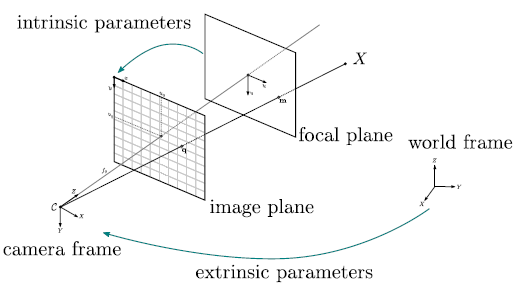
\includegraphics[width=0.7\linewidth]{image3.png}
%
%\caption{A pinhole-kameramodell. Forrás: http://openmvg.readthedocs.io/}
%\end{figure}
	
	
A kamerához definiálható egy kamera koordináta-rendszer. Ennek a koordináta-rendszernek az origójának a vetítés középpontját tekintjük, a z tengelye merőleges a vetítés síkjára. A kép koordináta-rendszer síkbeli koordináta-rendszer, a síkra vetített pontokat értelmezzük ebben. x és y tengelyei a kamera koordináta-rendszer tengelyeivel egyirányúak. Amennyiben homogén koordinátákkal jellemezzük a tér pontjait, mind a perspektív vetítés, mind a világ koordináta-rendszer és a kamera koordináta-rendszer közötti eltolás, forgatás mátrixszal kifejezhető: 

\begin{equation}
w\left[
\begin{array}{c}
u \\ v \\ 1
\end{array}
\right] = \left[ 
\begin{array}{ccc}
f_x & \gamma & u_0 \\
0 & f_y & v_0 \\
0 & 0 & 1
\end{array}
\right]\left[
\begin{array}{cccc}
r_{11} & r_{12} & r_{13} & t_1 \\
r_{21} & r_{22} & r_{23} & t_2 \\
r_{31} & r_{23} & r_{33} & t_3 \\
\end{array}
\right]\left[
\begin{array}{c}
x \\ y \\ z \\ 1
\end{array}
\right]
\end{equation}
 
A vetítés mátrixát kameramátrixnak hívjuk, a paramétereit pedig a kamera belső paramétereinek nevezzük. Mivel ezek a kamera rendeltetésszerű használata során nem változnak jelentősen, a kamera szerves részei, egyszeri kalibrálással meghatározhatók. A koordináta-rendszerek közti transzformáció paraméterei a külső paraméterek. Az összes paraméter meghatározható kellően nagy számú pontpár segítségével. A pontpárok alatt a világ koordináta-rendszerben ismert pozíciójú pontokat és azok kép koordináta-rendszerben megadott vetületét értjük. Az OpenCV-nek van olyan példakódja, amely elvégzi a kalibrációt, és kiszámítja a kérdéses mátrixokat.

A valóságban a pinhole kameramodell sajnos nem állja meg a helyét, a képet többféle torzítás terheli például abból adódóan, hogy nem vetítést alkalmazunk, hanem lencserendszert, valamint, hogy a detektoron elhelyezkedő pixelek gyártástechnológiája nem tökéletes. Ezeket a paramétereket most elhanyagoljuk, így a fenti összefüggésben a $\gamma$ paraméter 0 lesz.

	\section{Külső paraméterek meghatározása, PnP probléma}
	A kéz-szem kalibráció során szükség van a kamera külső paramétereinek ismeretére. Azt a feladatot, amely ismert térbeli helyzetű tárgypontok és a hozzájuk tartozó képi pontok alapján próbálja meghatározni a kamera külső paramétereit PnP, azaz Perspective-n-Point problémának nevezzük. 
	
Ennek egyik verziója a P3P algoritmus, amely csak 4 pontpárból számítja a paramétereket. Három pont kell ahhoz, hogy véges sok egyértelműen megoldást kapjunk (négy ponttal már túlhatározott lenne a feladat). A negyedik pontot az algoritmus arra használja fel, hogy a véges sok megoldás közül kiválassza a helyeset. Ezt úgy teszi meg, hogy a lehetséges négyféle megoldás közül azt választja, amelyikkel a negyedik pontot a képre vetítve a legkisebb hibát kapjuk a megadott képi ponthoz képest. Ezt aztán tetszőleges optimumkereséssel tovább lehet finomítani, pl. Levenberg-Marquardt eljárással. Ezt az eljárást használhatjuk akkor is, ha több, mint négy pont áll rendelkezése.
	
	\section{Kéz-szem kalibráció}
	A kéz-szem kalibráció során a robot megfogójának és a kamerának a relatív helyzetét kívánjuk meghatározni.

	Az ehhez használt módszer a belső paraméterek kalibrálásánál alkalmazotthoz hasonló, egy kalibrációs objektumról képeket készítünk, amelyen megkeressük a tárgy ismert pozíciójú pontjait. Az így kapott összefüggésekből számítjuk először a kamera külső paramétereit, majd az egyéb ismert paraméterek felhasználásával a kamera relatív helyzetét.	
	
	 A robotikában különböző koordináta-rendszereket használunk. A kalibráció során a következő koordináta-rendszereket használom:
	\begin{itemize}
	\item A robot bázis-koordinátarendszere, amelyik a nulladik, álló szegmenséhez van rögzítve. Betűjele: R (Robot)	
	\item A megfogó vagy szerszám koordináta-rendszere, amely a robot utolsó szegmensének végén található. Betűjele: T (Tool)
	\item A kamera koordináta-rendszere. Ennek a koordináta-rendszernek az origóját a pinhole modell alapján a vetítési pontba képzeljük el, a \textit{z} tengelye egybeesik az optikai tengellyel és a kamera nézési irányába mutat. A valóságban az optikai tengely és a lencse síkjának metszéspontjában található az origó. Betűjele: C (Camera)
	\item A tárgy-koordinátarendszer. Ez az a koordináta-rendszer, amiben a kalibráló objektum pontjainak koordinátáit értelmezzük. Nem kifejezetten lényeges, hogy hova tesszük, de az előbb említett koordinátákat numerikusan ismernünk kell ebben a koordináta-rendszerben. Betűjele: O(Object)
	\end{itemize}
	
	A $B$ koordináta-rendszerből az $A$ koordináta-rendszerbe való transzformáció a következőképpen írható fel homogén koordinátákban:
	\begin{equation}
	\label{trf-kifejt}
	\mathbf{T}_AB = 
	\left[
	\def\arraystretch{1.2}
	\begin{array}{c|c}
 	\mathbf{R}_AB & \mathbf{t}_AB \\
 	\hline
	\mathbf{0}^T & 1 \\
	\end{array}	
	\right]
	\end{equation}
	Itt $\mathbf{R}_AB$ 3x3-as rotációs mátrix, $\mathbf{t}_AB$ pedig oszlopvektor. A $\mathbf{t}_AB$ vektor az $A$ koordináta-rendszer origójából a $B$ koordináta-rendszer origójába mutat ($A$-ban felírva), míg $\mathbf{R}_AB$ oszlopai a $B$ koordináta-rendszer egységvektorai szintén $A$-ban felírva.
	A jelöléstechnikából következik, hogy $\mathbf{T}_AB^{-1} = \mathbf{T}_BA$
	
	A fent ismertetett koordináta-rendszerek közötti transzformációs lánc felírható:
	\begin{equation}\label{trf-lanc1}
	\mathbf{T}_CO\mathbf{T}_OR\mathbf{T}_RT\mathbf{T}_TC = \mathbf{I}
	\end{equation}
	Az egyes transzformációknak speciális tulajdonságaik vannak, amit kalibráláskor ki lehet (sőt kell) használni. A kamera a végberendezésre szilárdan van rögzítve, nem mozdul el. A robot is rögzítve van a gépalaphoz, amihez képest a kalibráló tárgy nem mozog a kalibráció során. Ez azt jelenti, hogy a $\mathbf{T}_OR$ és $\mathbf{T}_TC$ mátrixok nem változnak, ha a robotkart mozgatjuk. Ezen felül ismert a robotkar pozíciója a bázis-koordinátarendszerben, hiszen a robot irányítórendszere megoldja a direkt geometriai feladatot, valamint a PnP algoritmus megadja a kamera helyzetét a tárgy-koordinátarendszerben, így $\mathbf{T}_CO$ és $\mathbf{T}_RT$ mátrixok ismertek mindenkor.
	
	A kalibráció két lépésben történik. Az első lépésben a rotációs mátrixokat számítjuk ki, a másodikban a transzlációs vektorokat.
	\subsection{A rotációk becslése}
	A \eqref{trf-lanc1} egyenletet átalakítva kapjuk, hogy:
	\begin{equation}
	\label{trf-lanc2}
	\mathbf{T}_OC = \mathbf{T}_OR\mathbf{T}_RT\mathbf{T}_TC
	\end{equation}
	Ha az egész egyenletet beszorozzuk jobbról a nullvektorral:
	
	\begin{equation}
	\mathbf{T}_OC\left[ \begin{array}{c} 0 \\ 0 \\ 0 \\ 1 \end{array}	 \right] = \mathbf{T}_OR\mathbf{T}_RT\mathbf{T}_TC\left[ \begin{array}{c} 0 \\ 0 \\ 0 \\ 1 \end{array}	\right]
	\end{equation}		
	És elvégezzük a megfelelő szorzásokat:
	\begin{equation}
	\left[
	\begin{array}{c}
		\mathbf{t}_OC\\
		1
	\end{array}
	\right]	
	 = \mathbf{T}_OR 
	 \left[
	\begin{array}{c}
	\mathbf{R}_RT}t_{TC + \mathbf{t}_RT \\ 1
	\end{array}	
	 \right]
	\end{equation}
	Ebben az egyenletben számunkra ismeretlen a $\mathbf{T}_OR$ mátrix és a $\mathbf{t}_TC$ vektor. A kalibráció során készítünk $N$ darab képet, amelyekhez meghatározzuk a külső paramétereket, vagyis a $\mathbf{T}_OC$ mátrixot. Ezeket a képeket úgy készítjük el, hogy az $\mathbf{R}_RT$ mátrix állandó, vagyis két kép készítése között nem forgatjuk a kamerát, csak eltoljuk. Ekkor kiegészíthető a fenti egyenlet egy indexszel:
	\begin{equation}
	\left[
	\begin{array}{c}
		\mathbf{v}_OCi\\
		1
	\end{array}
	\right]	
	 = \mathbf{T}_OR 
	 \left[
	\begin{array}{c}
	\mathbf{R}_RT}t_{TC + \mathbf{t}_RTi \\ 1
	\end{array}	
	 \right] \quad i = 1..N
	\end{equation}
	Azok az ismeretlenek, illetve paraméterek, amik nem kaptak indexet, azok állandóak a képek készítése során. Vegyük a fenti $N$ darab egyenlet átlagát:
	\begin{equation}
	\left[
	\begin{array}{c}
	 	\frac{\sum \mathbf{t}_OCi}{N}\\
		1
	\end{array}
	\right]	
	 = \mathbf{T}_OR 
	 \left[
	\begin{array}{c}
	\mathbf{R}_RT}t_{TC + \frac{\sum \mathbf{t}_RTi}{N} \\ 1
	\end{array}	
	 \right]
	\end{equation}	
	Ha kivonjuk a két egyenletet egymásból, a következőt kapjuk:
		
	\begin{equation}
	\label{rot-trf1}
	\left[
	\begin{array}{c}
	 	\mathbf{t}_OCi - \frac{\sum \mathbf{t}_OCi}{N}\\
		0
	\end{array}
	\right]	
	 = \mathbf{T}_OR 
	 \left[
	\begin{array}{c}
	\mathbf{t}_RTi + \frac{\sum \mathbf{t}_RTi}{N} \\ 0
	\end{array}	
	 \right]
	\end{equation}	
	Bevezetjük, hogy:
	\begin{equation*}
	\begin{split}
	 	\overline{\mathbf{t}_OCi} &\coloneqq \mathbf{t}_OCi - \frac{\sum \mathbf{t}_OCi}{N} \\
	 	\overline{\mathbf{t}_RTi} &\coloneqq \mathbf{t}_RTi - \frac{\sum \mathbf{t}_RTi}{N} 
	 	\end{split}
	\end{equation*}
	Szemléletesen a felülvont változó az adott vektornak az összes vektor tömegközéppontjához képesti relatív helyzetét mutatja meg. Fontos látni, hogy ezek kiszámíthatók, ismerjük őket. \eqref{rot-trf1} írható a következő alakban is:
	\begin{equation}
	\left[
	\begin{array}{c}
	 	\overline{\mathbf{t}_OCi}\\
		0
	\end{array}
	\right]	
	 = \left[
	\def\arraystretch{1.2}
	\begin{array}{c|c}
 	\mathbf{R}_OR & \mathbf{t}_OR \\
 	\hline
	\mathbf{0}^T & 1 
	\end{array}	
	\right]
	 \left[
	\begin{array}{c}
	\overline{\mathbf{t}_RTi} \\ 0
	\end{array}	
	 \right]
	\end{equation}
	Ebből pedig:
	\begin{equation}
 	\overline{\mathbf{t}_OCi}	= \mathbf{R}_OR 	\overline{\mathbf{t}_RTi}
	\end{equation}
	$\mathbf{R}_OR$ kiszámítása tehát ekvivalens az kapott vektorpárok közti optimális rotáció kiszámításával. Optimális alatt azt a rotációt értem, amelyikkel a vektorpárok megfelelő tagját elfordítva a pár másik tagjához képesti legkisebb négyzetes hibaösszeget kapjuk.
	
	A Kabsch algortitmus pont ezt a problémát oldja meg, így én is ezt alkalmaztam. Az algoritmus a két vektorhalmaz közti koordinátánkénti kovariancia-mátrixot számítja ki, majd ennek SVD felbontásából határozza meg az optimális forgatást:
	\begin{equation}
	\label{kabsch-bigmat}
	\mathbf{P} \coloneqq \left[ \begin{matrix}
		\vdots \\
		\mathbf{{t_{RTi}}^T} \\
		\vdots
		\end{matrix} \right] \in \mathbb{R}^{N \times 3} , \quad
	\mathbf{Q} \coloneqq \left[ \begin{matrix}
		\vdots \\
		\mathbf{{t_{OCi}}^T} \\
		\vdots
		\end{matrix} \right] \in \mathbb{R}^{N \times 3} , \quad
		i = 1..N
	\end{equation}
	\begin{equation}
	\mathbf{A} = \mathbf{P}^T\mathbf{Q}
	\end{equation}
	\begin{equation}
	\mathbf{U \Sigma V}^T = \mathbf{A}
	\end{equation}
	\begin{equation}
	\mathbf{R}_OR = \mathbf{U}\left[
\begin{matrix}
1 & 0 & 0 \\
0 & 1 & 0 \\
0 & 0 & det(\mathbf{UV}^T) \\
\end{matrix}
	 \right]\mathbf{V}^T
	\end{equation}
	Ezután $\mathbf{R}_TC$ számítása történik: 
	\begin{equation}
	\mathbf{R}_TRi\mathbf{R}_RO\mathbf{R}_OCi = \mathbf{R}_TC\quad i = 1 .. N
	\end{equation}
	A bal oldalon található rotációs mátrixok "átlagát" kellene kiszámítani, ezt is a Kabsch algoritmussal oldom meg. Az algoritmusnak pontpárokra van szüksége. Ebben az esetben $3N$ darab vektorpárunk lesz, minden átlagolandó rotációhoz 3-3 vektorpár. Egy ilyen párhármas egyik tagja a rotációs mátrix megfelelő oszlopvektora, a másik tagja pedig a neki megfelelő egységvektor ($\left[1\:0\:0 \right]^T $, $\left[0\: 1\: 0 \right]^T $, vagy $\left[0\: 0\: 1 \right]^T $). Ekkor a \eqref{kabsch-bigmat}-ben definiált mátrixok a következő alakot öltik:
	\begin{equation}
	\mathbf{P} \coloneqq \left[ \begin{matrix}
		\vdots \\
		\mathbf{R}_TRi\mathbf{R}_RO\mathbf{R}_OCi \\
		\vdots
		\end{matrix} \right], \quad
	\mathbf{Q} \coloneqq \left[ \begin{matrix}
		\vdots \\
		\mathbf{I} \\
		\vdots
		\end{matrix} \right], \quad
		i = 1..N
	\end{equation}
	ahol $\mathbf{I}$ a $3\times 3$-as egységmátrix.
	
	Így a rotációk átlagát véve a Kabsch algoritmussal megkaphatjuk az $\mathbf{R}_TC$ mátrixot.
	\subsection{A transzlációk becslése}
	Ha kifejtjük a \eqref{trf-lanc2} egyenletet \eqref{trf-kifejt} szerint:
	\begin{equation}
	\left[ 	\def\arraystretch{1.2} \begin{array}{c|c}
 	\mathbf{R}_OC & \mathbf{t}_OC \\ \hline
	\mathbf{0}^T & 1 \\
	\end{array}	\right] = 	
	\left[ \def\arraystretch{1.2} \begin{array}{c|c}
 	\mathbf{R}_OR & \mathbf{t}_OR \\ \hline
	\mathbf{0}^T & 1 \\
	\end{array}	\right]	
	\left[ \def\arraystretch{1.2} \begin{array}{c|c}
 	\mathbf{R}_RT & \mathbf{t}_RT \\ \hline
	\mathbf{0}^T & 1 \\
	\end{array}	\right]	
	\left[ \def\arraystretch{1.2} \begin{array}{c|c}
 	\mathbf{R}_TC & \mathbf{t}_TC \\ \hline
	\mathbf{0}^T & 1 \\
	\end{array}	\right]
	\end{equation}
	Összeszorozva a jobb oldalt:
	\begin{equation}	
	\left[ \def\arraystretch{1.2} \begin{array}{c|c}
 	\mathbf{R}_OC & \mathbf{t}_OC \\ \hline
	\mathbf{0}^T & 1 \\
	\end{array}	\right] = 
	\left[ \def\arraystretch{1.2} \begin{array}{c|c}
 	\mathbf{R}_OR}R_{RT}R_{TC & \mathbf{R}_OR}R_{RT}t_{TC+\mathbf{R}_OR}t_{RT + \mathbf{t}_OR \\ \hline
	\mathbf{0}^T & 1 \\
	\end{array}	\right]
	\end{equation}
	Ebben a fázisban a készített képek számát jelöljük $M$-mel. Ebből, ha bevezetjük az indexet a változó paraméterekhez , kapjuk, hogy:
	\begin{equation}
	\mathbf{t}_OCi = \mathbf{R}_OR}R_{RTi}t_{TC+\mathbf{R}_OR}t_{RTi + \mathbf{t}_OR \quad i=1..M
	\end{equation}
	Figyeljük meg, hogy most már a megfogó orientációját, azaz az $\mathbf{R}_RTi$ mátrixot is változtatjuk a képek készítése során. A fenti egyenletben az ismeretlenek a $\mathbf{t}_TC$ és $\mathbf{t}_OR$ vektorok. Átrendezve az egyenletet:
	\begin{equation}
	\mathbf{R}_OR^{-1} \mathbf{t}_OCi -  \mathbf{t}_RTi =  \mathbf{R}_RTi\mathbf{t}_TC+\mathbf{R}_OR^{-1}\mathbf{t}_OR
	\end{equation}
	Bevezetve:
	
	\begin{equation}
	\begin{split}
	\mathbf{p_i} &\coloneqq \mathbf{R}_OR^{-1} \mathbf{t}_OCi -  \mathbf{t}_RTi \\
	\mathbf{A_i} &\coloneqq  \mathbf{R}_RTi\\
	\mathbf{B} &\coloneqq  \mathbf{R}_OR^{-1}
	\end{split}
	\end{equation}
	
	Kapjuk, hogy:
	\begin{equation}
	\mathbf{p_i} =  \mathbf{A_i}\mathbf{t}_TC+\mathbf{B}\mathbf{t}_OR
	\end{equation}
	Ha az összes $M$ egyenletet egybefoglaljuk:
	\begin{equation}
	\mathbf{Cx} = \mathbf{k}
	\end{equation}
	ahol:
	\begin{equation}
	\mathbf{x} \coloneqq \left[ \begin{matrix} \mathbf{t}_TC \\ \mathbf{t}_OR\end{matrix}	 \right], \quad
	\mathbf{C} \coloneqq  \left[ \begin{array}{cc} \multicolumn{2}{c}{\vdots} \\ \mathbf{A_i} & \mathbf{B} \\ \multicolumn{2}{c}{\vdots}  \end{array} \right], \quad
	\mathbf{k} \coloneqq  \left[ \begin{matrix} \vdots \\ \mathbf{p_i} \\ \vdots \end{matrix} \right] 
	\end{equation}
	\begin{equation*}
	\mathbf{x} \in \mathbb{R}^{6 \times 1}, \quad
	\mathbf{C} \in \mathbb{R}^{3M \times 6}, \quad
	\mathbf{k} \in \mathbb{R}^{3M \times 1}, \quad
	i = 1..M
	\end{equation*}
	Innen a pszeudoinverz segítségével az optimális megoldás számolható:
	\begin{equation}
	\hat{\mathbf{x}} = \left(\mathbf{C}^T \mathbf{C}\right)^{-1}\mathbf{C}^T\mathbf{k}
	\end{equation}
	\section{Eredmények}
	A kalibráló algoritmust a \ref{img-gui}. ábrán látható sakktáblamintával futtattam le. Az első lépésben azonos rotáció mellett 10-10 mérést végeztem minden tengely mentén elmozdítva a kamerát. A második fázisban a sakktáblára nagyjából ±15°-os szögből néztem rá, két tengely mentén mozgatva a kamerát.
	
	 A rotáció meghatározásának pontossága igen jó volt, viszont a megfogó és a kamera közti eltolást nem tudta meghatározni pontosan. A PnP algoritmus az objektum kamerától való távolságára nem kifejezetten érzékeny, nagy hibát tud véteni, ezért a kalibráló algoritmus is rossz adatokból dolgozik. A kamera oldalirányú elmozdulását szépen érzékeli a kalibráció, a z irányú elmozdulást viszont több 100\%-os hibával tudja csak meghatározni. 
	
	\section{Továbbfejlesztési lehetőségek}
	A kalibrálásra több módszer is rendelkezésre áll, valószínűleg fejlettebbek, mint az általam implementált, lehet, hogy azokkal kisebb hiba is megvalósítható.
	
	A most használt algoritmus is javítható lenne, ha a kamerahelyzet-meghatározásnál különböző bizonytalanságok figyelembe vételével kiegészítenénk az algoritmust.
	
	A nagy kalibrálási hiba okozója a kis látószög is lehet, ezt növelve talán nagyobb pontosság érhető el.
	
	\section{Forrásjegyzék}

\begin{enumerate}
\item Gao, Xiao-Shan; Hou, Xiao-Rong; Tang, Jianliang; Cheng, Hang-Fei (2003). "Complete Solution Classification for the Perspective-Three-Point Problem"

\item Kabsch, W. (1976). A solution for the best rotation to relate two sets of vectors. Acta Crystallographica Section A, 32(5), pp.922-923.
\end{enumerate}

\end{document}
